\documentclass{article}
\usepackage[utf8]{inputenc}
\usepackage{amsmath}
\usepackage{enumitem}
\usepackage{graphicx} 
\author{Knoll Alexander & Phillip Durry}
\title{Numerik 2: Abgabe 1}
\newcommand{\pp}[1]{\phantom{#1}}
\renewcommand{\theenumi}{\Alph{enumi}}
\newcommand\Section[1]{ %
  \addtocontents{toc}{\protect\setcounter{tocdepth}{0}}
  \subsubsection*{#1}
  \addtocontents{toc}{\protect\setcounter{tocdepth}{3}}}


\begin{document}

\maketitle
\newpage
\tableofcontents
\newpage

\section{Aufgabe 1}

\section{Aufgabe 2}

	\subsection{Mehrschrittverfahren untersuchen}
	
		Untersuchen Sie für die folgenden Mehrschrittverfahren, ob sie mindestens von der Ordnung 2
		sind (d. h. lokale Konsistenzordnung 3 besitzen) und ob sie stabil sind:
	
		\begin{enumerate}[label=(\alph*)]
			\item  $y_{i+1} = y_{i-1} + 2hf_{i}$ 
			\item  $y_{i+1}  = 3y_{i} - 2y_{i-1} + \frac{h}{12}[7f_{i+1} - 8f_{i} - 11f_{i-1}] $ 
			\item  $y_{i+1} = \frac{4}{3}y_{i} - \frac{1}{3}y_{i-1} + \frac{h}{9}[4f_{i+1} + 4f_{i} - 2f_{i-1}]$ 
		\end{enumerate}
		
		Zunächst sollen die Verfahren auf Stabilität hin untersucht
	
	\subsection{Verfahren implementieren}
	
		Implementieren Sie das erste der drei Verfahren sowie das Verfahren
		
		\begin{align*}
			y_{i+1} = \frac{4}{3}y_{i} - \frac{1}{3}y_{i-1} + \frac{2h}{3}f_{i+1}
		\end{align*}
		
		und verwenden Sie bei letzerem ein geeignetes Verfahren zum Lösen des nichtlinearen Gleichungssystems.
		
	\subsection{Numerische Lösung}
	
		Berechnen Sie (mit Python) numerische Lösungen mit $h = 1; 10^{-1} ; 10^{-2} , ...$ ausgehend von den exakten Startwerten für $y(0)$ und $y(h)$ für den Wert $y(10)$ und bestimmen Sie jeweils die Fehler.Bestimmen Sie daraus auch die Fehlerordnung und vergleichen Sie sie mit Ihrem theoretischenErgebnis.
		
	\subsection{Anfangswertproblem untersuchen}
	
		Gegeben ist das Anfangswertproblem
	
		\begin{align}
			\dot{y} = -2y(t) + 1 , y(0) = 1
		\end{align}
		
		Bestimmen sie die exakte Lösung des AWPs und vergleichen Sie sie mit der numerischen.

		\subsubsection{Analytische Lösung}
		
			Zunächste muss Gleichung (1) in Standart Notation gebracht werden, welche gegeben ist durch:
			
			\begin{align*}
				\dot{y} + p(t) = Q(t)
			\end{align*}
			
			Somit kann Gleichung (1) überführt werden in
			
			\begin{align}
				\dot{y} + 2y = 1
			\end{align}
			
			Eine allgemeine lösung zu einer Gleichung in Standart Notation kann mithilfe folgender ausdrücke bestimmt werden
			
			\begin{align*}
				u(x) = e^{\int p(x) dt} \\
				\frac{d}{dt}(uy) = Q(t)
			\end{align*}
			
			Angewandt auf Gleichung (2) erhält man einen Ausdruck welcher durch beidseitiges integrieren und weiterem umformen, die
			allgemeine Lösung des Problems beschreibt.
			
			\begin{align*}
				u = e^{\int 2 dt}\\
				\frac{d}{dt}(e^{2t}y) = e^{2t} && | \int \\
				\int \frac{d}{dt}(e^{2t}y) = \int e^{2t} \\
				e^{2t}y = \frac{1}{2}e^{2t} + C && | \div e^{2t} \\
				y = \frac{1}{2} + \frac{C}{e^{2t}} \\
				y = \frac{1}{2} + Ce^{-2t}
			\end{align*}
			
			Einbeziehen der Anfangsbedingung $y(0) = 1$ liefert die exakte Lösung des Problems
			
			\begin{align*}
				y(0) = \frac{1}{2} + C*e^{-2*0} \\
				1 = \frac{1}{2} + C && | - \frac{1}{2} \\
				\frac{1}{2} = C
			\end{align*}
			
			Und somit die exakte Lösung
			
			\begin{align}
				y(t) = \frac{1}{2}e^{-2t} + \frac{1}{2}
			\end{align}
			
			\begin{figure}[htbp] 
			  \centering
			     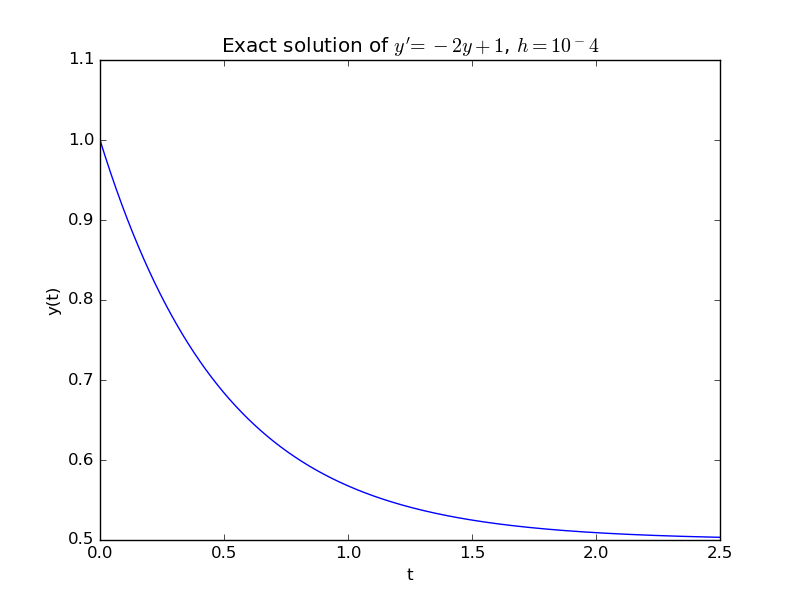
\includegraphics[width=0.7\textwidth]{analytic_solution.png}
			  \caption{Analytische lösung im Intervall [0; 2,5]}
			  \label{fig:Bild1}
			\end{figure}
			
			Wenn nun Störungungen in die Anfangsbedingung eingeführt werden, kann man das Problem auf stabilität untersuchen. Hierfür wird
			,ausgehend von der allgemeinen lösung, eine exakte Lösung unter verwendung von $y(0) = 1 + \epsilon$ bestimmt.
			
			\begin{align*}
				y_{\epsilon}(t) = (\frac{1}{2} + \epsilon)e^{-2t} + \frac{1}{2}
			\end{align*}
			
			Es ist leicht zu sehen dass für sehr kleine $\epsilon$, die lösung keine größeren abweichungen erfährt.
			Somit kann die Lösung als Stabil bezeichnet werden. 
			
		\subsubsection{Numerische Lösung}
		
			Als folge der stabilität des AWPs, ist es sehr wahrscheinlich dass Einschrittverfahren für ausreichend kleine $h$ gegen die Lösung des Problems konvergieren. Deshalb soll im folgend der vergleich dreier Verfahren, die Schrittweite $h=0,5$ genutzt werden. Dies liefert eine bessere visuelle darstellung der tatsächlichen unterschiede der genutzen Verfahren. Genutzt werden dass implizite und explizite Euler-Verfahren als auch dass Adams-Moultan-Verfahren (Ordnung 2).
			
			\Section{Expliziter Euler}
			
				Das Verfahren wird beschrieben durch
				
				\begin{align*}
					u_{i+1} = u_{i} + hf_{i}
				\end{align*}
				
				angewandt auf Gleichung (1) erhält man
				
				\begin{align*}
					y_{i+1} = y_{i} + h(-2y_{i}+1) \\
					y_{i+1} = (1-2h)y_{i} + h
				\end{align*}
			
			\Section{Impliziter Euler}
			
				Das implizite verfahren lautet wie folgt.
				
				\begin{align*}
					u_{i+1} = u_{i} + hf_{i+1}
				\end{align*}
				
				Da $y' = f(t, y)$ bekannt ist es möglich dass verfahren durch umformungen auf eine einfach
				auswertbare Form zu bringen. Andernfalls wäre es notwendig in jedem iterations-schritt ein passendes
				Lösungsverfahren anzuwenden, wie beispielsweise dass Newton-Verfahren oder dass Sekanten-Verfahren.
				
				\begin{align*}
					y_{i+1} = y_{i} + h(-2y_{i+1}+1) \\
					y_{i+1} = y_{i} - 2hy_{i+1} + h  && | +2hy_{i+1} \\
					(1+2h)y_{i+1} = y_{i} + h && | \div(1+2h) \\
					y_{i+1} =  \frac{y_{i} + h}{1+2h}
				\end{align*} 
			
			\Section{Adams-Moultan}
			
				Dieses Verfahren existieren in verschiedenen Variationen. In diesem Fall wird die Methode der 2. Ordnung verwendet.
				
				\begin{align*}
					u_{i+1} = u_{i} + \frac{h}{2}[f_{i+1} + f_{i}]
				\end{align*}
				
				Wie bereits beim implizieten Euler Verfahren, ist es möglich die gleichung in eine einfach auswertbare form zu
				bringen.
				
				\begin{align*}
					y_{i+1} = y_{i} + \frac{h}{2}[-2y_{i+1} + 1 - 2y_{i+1} + 1] \\
					y_{i+1} = y_{i} - hy_{i+1} - hy_{i} + h && | +hy_{i+1} \\
					(1+h)y_{i+1} = (1-h)y_{i} + h && | \div(1+h) \\
					y_{i+1} = \frac{(1-h)y_{i}+h}{1+h}
				\end{align*}
				
			
			\Section{Vergleich}
			
				Unter einbezug von Python werden die resultate visualisiert.
				
				\begin{figure}[htbp] 
					\centering
					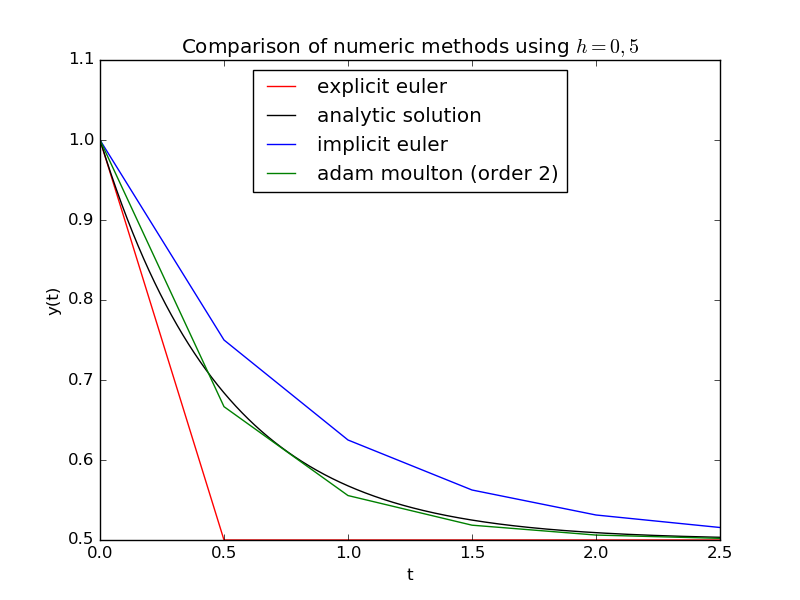
\includegraphics[width=0.7\textwidth]{numeric_plots.png}
					\caption{Vergleich der Numerischen Lösungen mit der Analytischen}
					\label{fig:Bild2}
				\end{figure}
			
				Die Grafik zeigt deutlich, dass jedes der angewandten Verfahren letztendlich gegen die Lösung konvergiert.
				Jedoch konvergieren die Einschritt-Verfahren wesentlich langsamer als das Adams-Moultan-Verfahren, welches 
				selbst für recht große $h$ einen guten eindruck macht. Weiterhin scheint es so als würde dass expliziete Euler-Verfahre direkt nach dem ersten iterations schritt auf 0 fallen, wodurch es unbrauchbar wird. Abhilfe schafft eine kleinere Wahl von $h$.
				
				\newpage
				
				\begin{figure}[htbp] 
					\centering
					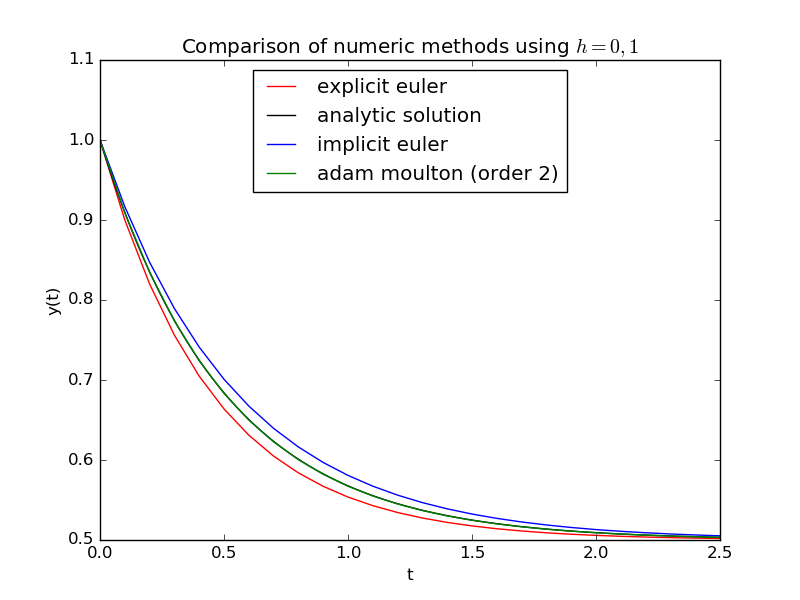
\includegraphics[width=0.7\textwidth]{numeric_plots2.png}
					\caption{Numerische Lösungen mit kleinerem h}
					\label{fig:Bild3}
				\end{figure}
				
				In der obigen Abbildung wird deutlich, wie gut das Adams-Moultan-Verfahren für das AWP geeignet ist.
	
\end{document}